\documentclass{jsarticle}
\usepackage[dvipdfmx]{graphicx}
\usepackage{listings}
\usepackage{afterpage}
\begin{document}
\title{課題3 2値化画像におけるしきい値の変化}
\author{13EC060 武澤 裕介}
\maketitle
\begin{abstract}
まずmatlabを用いて2値化画像を作成する。しきい値を変化させて画像の変化を考察する。
\end{abstract}
\section{しきい値の変化}
まず、今回使用する原画像を図1に示す。
\begin{lstlisting}[basicstyle=\ttfamily\footnotesize, frame=single]
ORG=imread( uigetfile('*')); % 原画像の入力
ORG= rgb2gray(ORG); % カラー画像を白黒濃淡画像へ変換
imagesc(ORG); colormap(gray); colorbar; % 画像の表示
pause;
 \end{lstlisting}
を用いてまず入力画像のグレースケール画像を表示させる。

\begin{figure}[htbp]
 \begin{center}
  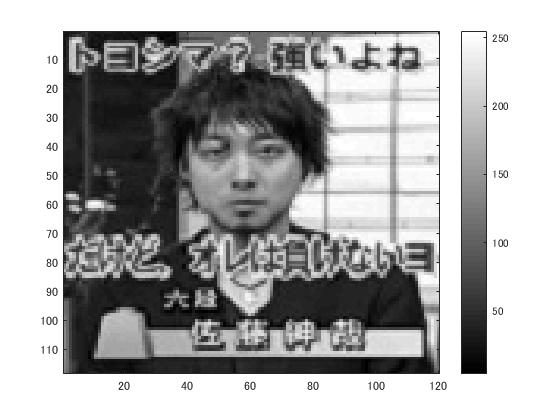
\includegraphics[width=10cm]{kadai3-0.jpg}
 \end{center}
 \caption{原画像}
\end{figure}

次に輝度値が64以上の画素を1,その他を0に変換として画像の2値化を行う。
\begin{lstlisting}[basicstyle=\ttfamily\footnotesize, frame=single]
IMG = ORG > 64;
imagesc(IMG); colormap(gray); colorbar;
pause;
 \end{lstlisting}
としきい値を設定する。

\begin{figure}[htbp]
 \begin{center}
  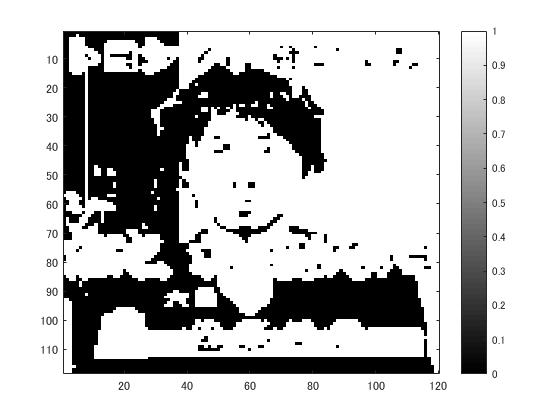
\includegraphics[width=10cm]{kadai3-1.jpg}
 \end{center}
 \caption{しきい値64の2値化画像}
\end{figure}

次に輝度値が96以上の画素を1,その他を0に変換として画像の2値化を行う。
\begin{lstlisting}[basicstyle=\ttfamily\footnotesize, frame=single]
IMG = ORG > 96;
imagesc(IMG); colormap(gray); colorbar;
pause;
\end{lstlisting}
としきい値を設定する。

\begin{figure}[htbp]
 \begin{center}
  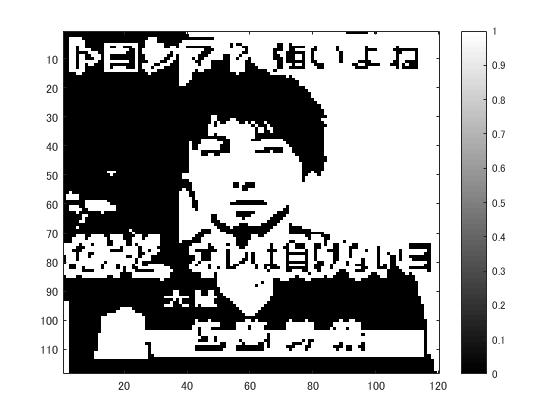
\includegraphics[width=10cm]{kadai3-2.jpg}
 \end{center}
 \caption{しきい値96の2値化画像}
\end{figure}

最後に輝度値が128以上の画素を1,その他を0に変換として画像の2値化を行う。
\begin{lstlisting}[basicstyle=\ttfamily\footnotesize, frame=single]
IMG = ORG > 128;
imagesc(IMG); colormap(gray); colorbar;
pause;
\end{lstlisting}
としきい値を設定する。
\begin{figure}[htbp]
 \begin{center}
  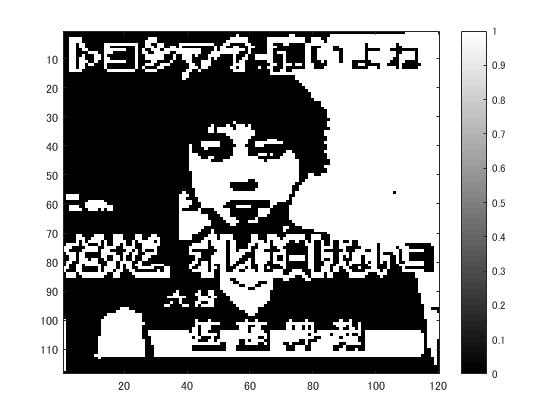
\includegraphics[width=10cm]{kadai3-3.jpg}
 \end{center}
 \caption{しきい値128の2値化画像}
\end{figure}

\newpage

最後に輝度値が192以上の画素を1,その他を0に変換として画像の2値化を行う。
\begin{lstlisting}[basicstyle=\ttfamily\footnotesize, frame=single]
IMG = ORG > 192;
imagesc(IMG); colormap(gray); colorbar;
pause;
\end{lstlisting}
としきい値を設定する。
\begin{figure}[htbp]
 \begin{center}
  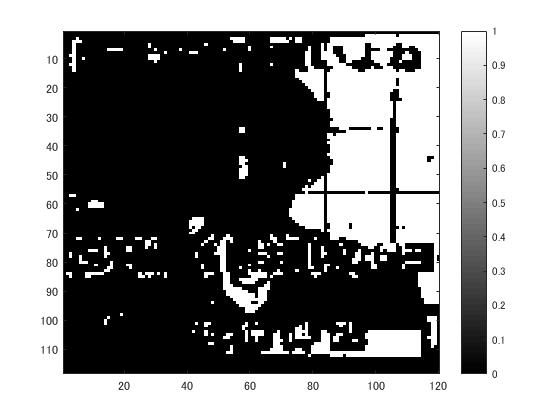
\includegraphics[width=10cm]{kadai3-4.jpg}
 \end{center}
 \caption{しきい値192の2値化画像}
\end{figure}

\section{考察}
今回2値化画像のしきい値を変化させて画像の変化を観察したが、図2から図5につれて2値化における0の画素の領域が増えていくので、輝度値が高い方が明るく見え、低いほど暗く見えている事がわかる。
\end{document}